\documentclass[11pt]{article}
\usepackage{amsthm}
\usepackage{xspace}
\usepackage{siunitx}
\usepackage{booktabs}
\usepackage{miscdoc,multirow,bigstrut,bigdelim,colortbl}
\usepackage{setspace}
\usepackage{listings}
\usepackage{graphicx}
\usepackage{amsmath}
\usepackage{subfig}
\usepackage{intcalc}
\usepackage{polynomial}
\usepackage{polynom}


\DeclareUnicodeCharacter{2212}{-}
\begin{document}
\title{Homework-3}
\author{Mustafa Tokat}
\maketitle
\section{Introduction}
I analyzed several paper together with our lectures during my homework. I studied to understand those, followed step by step entire of the process.
 Now, we have to 5 problems and will try to solve step by step these.
\section{Analysis of problems}
\subsection{Problem 1}
 
\textbf{(1) IP(1248842112488421):}
In this process only place of values change, not themselves of values. We can figure out it with a little codes snippet.
\lstset{language=Python}
\lstset{frame=lines}
\lstset{caption={for to permute IP}}
\lstset{label={lst:code_direct}}
\lstset{basicstyle=\footnotesize}
\begin{lstlisting}
  def permutation(ptext, table, nbit):
    permuted = ""
    for i in range(0, nbit):
        permuted = permuted + ptext[table[i]-1]
    return permuted
\end{lstlisting}
\underline{Result: 2211448844882211 }\\

\bigskip\textbf{(2) E(84211248): }
By changing the parameters of the code snippet above, we can find the E permutation.\\
\underline{Result: 4081028A4251}\\

\bigskip\textbf{(3) P(12488421): }
Similarly;\\
\underline{Result: 41010C4A}\\

\newpage\textbf{(4) Si(110011) for i = 1; 2; : : : ; 8:}
We can use below codes: 
\lstset{language=Python}
\lstset{frame=lines}
\lstset{caption={for to S-Box}}
\lstset{label={lst:code_direct}}
\lstset{basicstyle=\footnotesize}
\begin{lstlisting}
  for i in range(0,8):
        val = S_BOX[i][3][9]
        sboxTable = sboxTable + dec2bin(val)
\end{lstlisting}
\underline{Result: 1011 0110 1111 0100 1111 1110 0101 1100 }\\




\subsection{Problem 2}
\subsubsection{}
\textbf{Suppose that $K_{1}$ = $K_{2}$ = · · · = $K_{16}$. Show that all bits in $C_{1}$ are equal and all bits in $D_{1}$
are equal}\\
 
Key scheduling is exactly independent a process from making ciphertext. The first half of the 56-bit key is left, also its second half 
is right are called as. At the same time, entire of the this process is logic and can be inversion.Now, we can establish the logical connection. 
$K_{i}$ values is generated after from come side by side $C_{i}$  and $D_{i}$ values,and this process cocnsists two of two steps.
(a) Left-shift and (b) PC2. $C_{i}$  and $D_{i}$ values are make left-shift for each round. After new values are permuted with PC2. According to our suppose,
if entire of the our keys are same, this mean entire of  $C_{i}$ are same and also $D_{i}$ are same. I encrypted the 'CryptoEn' to explain with an example.
The result is as follow.\\
\begin{figure}[!h]
  \centering
  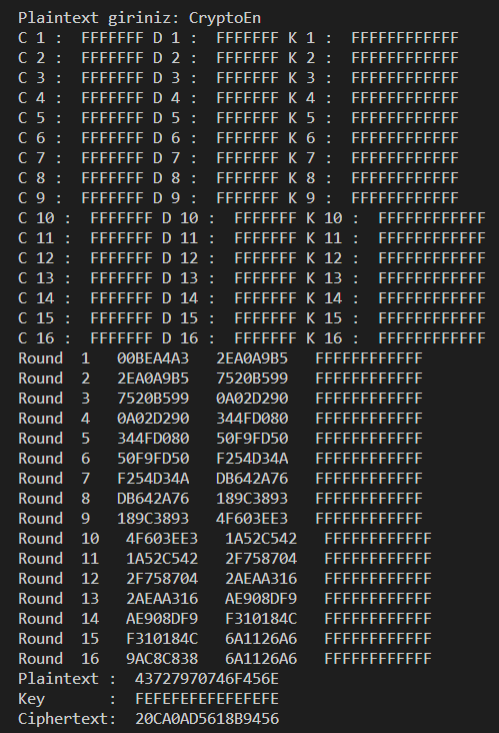
\includegraphics[width=0.7\textwidth]{Screenshot_3.png}
  \caption{if $K_{i}$ values are the same }
  \label{fig:boat1}
\end{figure}

\newpage
\subsubsection{}\textbf{Show that there are exactly 4 DES keys for which all round keys are the same. They are
called weak DES keys.}\\


If we carefully analyze, we can see that dropped 48-bit of PC2 permutation cocnsists its first half from 1-28nth bits and also second half
from 29-48nth bits. Therefore, we can easily say that first 24 bits of the $K_{i}$ values formed from PC2 are left and second 24 bits of the $K_{i}$ values
formed from PC2 are right. The results is follow:

\begin{figure}[ht!]
  \centering
  \subfloat[1F1F1F1F 0E0E0E0E]
    {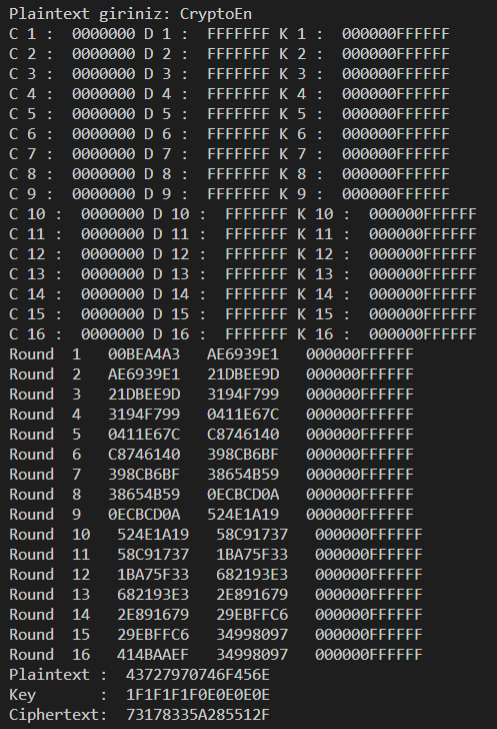
\includegraphics[width=0.4\textwidth]{Screenshot_1.png}}\quad
  \subfloat[E0E0E0E0 F1F1F1F1]
    {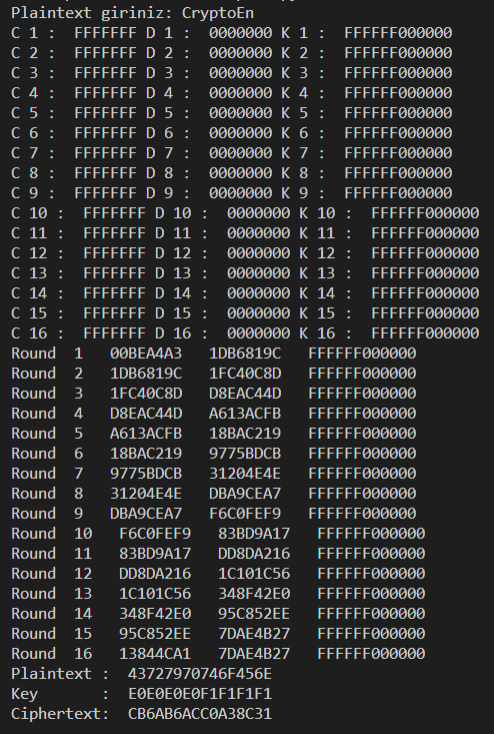
\includegraphics[width=0.4\textwidth]{Screenshot_2.png}}\\
  \subfloat[FEFEFEFE FEFEFEFE]
    {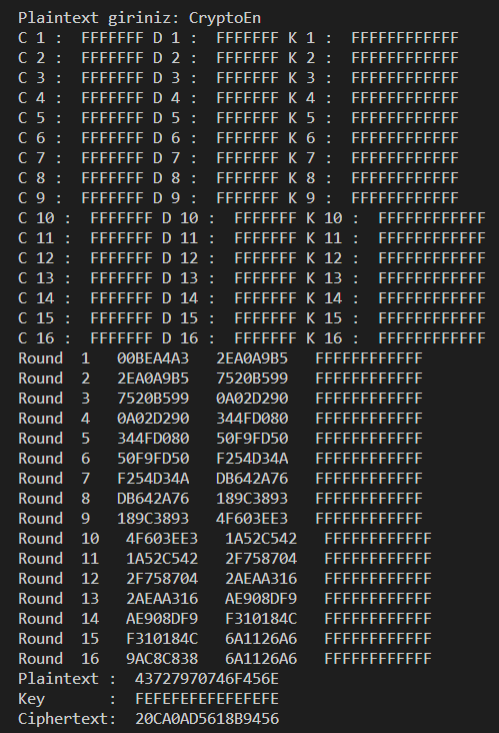
\includegraphics[width=0.4\textwidth]{Screenshot_3.png}}\quad
  \subfloat[01010101 01010101]
    {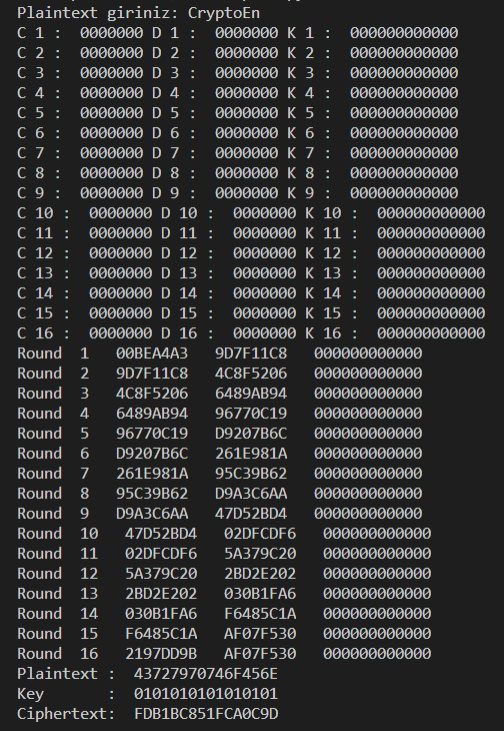
\includegraphics[width=0.4\textwidth]{Screenshot_4.png}}
  \caption{weak Keys}
  \label{fig:Weak keys}
\end{figure}


\clearpage
\subsubsection{}\textbf{Determine these 4 weak DES keys.}\\

The 4 weak keys were published by NIST in January 2012\footnote{Recommendation for the Triple Data Encryption Algorithm (TDEA)
Block Cipher, NIST, January 2012, p.11}. These are:\\
\begin{itemize}
  \item 01010101 01010101
  \item FEFEFEFE FEFEFEFE
  \item E0E0E0E0 F1F1F1F1
  \item 1F1F1F1F 0E0E0E0E
\end{itemize}


\subsection{Problem 3}
\textbf{There are other modes of block cipher besides the ones we have learned. One of these modes
is named Plaintext Block Chaining (PBC) Mode. On the encryption side, the following is
executed to obtain the nth ciphertext: Cn := $E_{k}$($M_{n}$) $\oplus$  $M_{n-1}$. Suppose that we need to
encrypt M1,...,M5 using the PBC mode. Show the explicit formulas to obtain C1,...,C5.
What do you need to use for M0? Also, show the steps on the decryption side to obtain
M1,...,M5.}\\

$M_{0}$ is Initialization Vector(IV). In this case, we can constitue to encryption and decryption formulas: \\

  \begin{itemize}
    \item for encryption:
    \begin{itemize}
      \item[$\circ$] $C_{1}$ = $E_{k}$($M_{1}$) $\oplus$ IV
      \item[$\circ$] $C_{2}$ = $E_{k}$($M_{2}$) $\oplus$ $M_{1}$
      \item[$\circ$] $C_{3}$ = $E_{k}$($M_{3}$) $\oplus$ $M_{2}$
      \item[$\circ$] $C_{4}$ = $E_{k}$($M_{4}$) $\oplus$ $M_{3}$
      \item[$\circ$] $C_{5}$ = $E_{k}$($M_{5}$) $\oplus$ $M_{4}$
    \end{itemize}\
  \end{itemize}

Interestingly, we  continue toward  from start to end in order to decryption, because decryption process continue toward 
from end to start in some algorithm.

\newpage\begin{itemize}
  \item for decryption:
  \begin{itemize}
    \item[$\circ$] $M_{1}$ = $D_{k}$($C_{1}$) $\oplus$ IV
    \item[$\circ$] $M_{2}$ = $D_{k}$($C_{2}$) $\oplus$ $C_{1}$
    \item[$\circ$] $M_{3}$ = $D_{k}$($C_{3}$) $\oplus$ $C_{2}$
    \item[$\circ$] $M_{4}$ = $D_{k}$($C_{4}$) $\oplus$ $C_{3}$
    \item[$\circ$] $M_{5}$ = $D_{k}$($C_{5}$) $\oplus$ $C_{4}$
  \end{itemize}
\end{itemize}





\subsection{Problem 4}
\textbf{Consider the AES/Rijndael algorithm and its Galois field GF($2^{8}$)}
\subsubsection{Compute the sum (a7) + (5c) in GF($2^{8}$)}

At first, we should convert these hex values to binary numbers.\\

\begin{center}
  (a7) = 1 0 1 0 0 1 1 1
\end{center}

\begin{center}
  (5c) = 0 1 0 1 1 1 0 0
\end{center}



After, we should write to binary numbers as polynomial and should sum to this polynomials(indeed XOR);\\


\begin{center}
  ($x^{7}$ + $x^{5}$ + $x^{2}$ + $x^{1}$ + 1) $\oplus$ ($x^{6}$ + $x^{4}$ + $x^{3}$ + $x^{2}$)\\
\end{center}

\begin{center}
  = $x^{7}$ + $x^{6}$ + $x^{5}$ + $x^{4}$ + $x^{3}$ + $x^{1}$ + 1\\
\end{center}


Now, we should convert these polynomials to binary numbers.\\

\begin{center}
  = $\underbrace{1 1 1 1}_\text{f}$ $\underbrace{1 0 1 1}_\text{b}$
\end{center}


\underline{Result} = (a7) + (5c) = (fb)

\subsubsection{Compute the product (a7) × (5c) in GF($2^{8}$)}

At first, we should convert these hex values to binary numbers.\\

(a7) = 1 0 1 0 0 1 1 1\\

(5c) = 0 1 0 1 1 1 0 0\\

Besides, I want to solve with two method.\\

\underline{First method}\\

\begin{center}
  ($x^{7}$ + $x^{5}$ + $x^{2}$ + $x^{1}$ + 1) $\mathsf{X}$ ($x^{6}$ + $x^{4}$ + $x^{3}$ + $x^{2}$)\\
\end{center}

\begin{center}
  = $x^{13}$ + $x^{11}$ + $x^{10}$ + $x^{9}$ + $x^{11}$ + $x^{9}$ + $x^{8}$ + $x^{7}$ + $x^{8}$ + $x^{6}$ + $x^{5}$ + $x^{4}$ +
  $x^{7}$ + $x^{5}$ + $x^{4}$ + $x^{3}$ + $x^{6}$ + $x^{4}$ + $x^{3}$ + $x^{2}$\\ 
\end{center}

\begin{center}
  = $x^{13}$ + $x^{10}$ + $x^{4}$ + $x^{2}$\\
\end{center}

And now, I will divide to p(x) = $x^{8}$ + $x^{4}$ + $x^{3}$ + $x^{}$ + 1\\

\polylongdiv[style=D]{x^{13}+x^{10}+x^{4}+x^{2}}{x^{8}+x^{4}+x^{3}+x+1}\\

=$x^{5} + x^{4} + x^{2}$ + 1\\

Now, we will convert it to binary numbers;\\

= $\underbrace{0 0 1 1}_\text{3}$$\underbrace{0 1 0 1}_\text{5}$\\

\underline{Result:} (a7) x (5c) = (35)\\ 

\underline{Second method}\\

At first, we are convert to $x^{13}$ + $x^{10}$ + $x^{4}$ + $x^{2}$ polynomial to binary numbers and will write its under;\\

1 0 0 1 0 0 0 0 0 1 0 1 0 0 \\

\underline{1 0 0 0 1 1 0 1 1} \\

0 0 0 1 1 1 0 1 1 1 0 1 0 0 \\

\underline{0 0 0 1 0 0 0 1 1 0 1 1} \\

0 0 0 0 1 1 0 0 0 1 1 0 \\

\underline{0 0 0 0 1 0 0 0 1 1 0 1 1 }\\

0 0 0 0 0 1 0 0 1 0 1 1 1 0\\

\underline{0 0 0 0 0 1 0 0 0 1 1 0 1 1}\\

0 0 0 0 0 0 0 0 1 1 0 1 0 1\\

We take to last 8 numbers and convert it hex number;\\

$\underbrace{0 0 1 1}_\text{3}$ $\underbrace{ 0 1 0 1}_\text{5} $


\underline{Result: }(a7) x (5c) = (35)\\


\subsubsection{Compute S(a7)}

I will explain in details solving of this question in  next question, for this reason I prefer to solve by looking to the table. \\

\begin{figure}[!h]
  \centering
  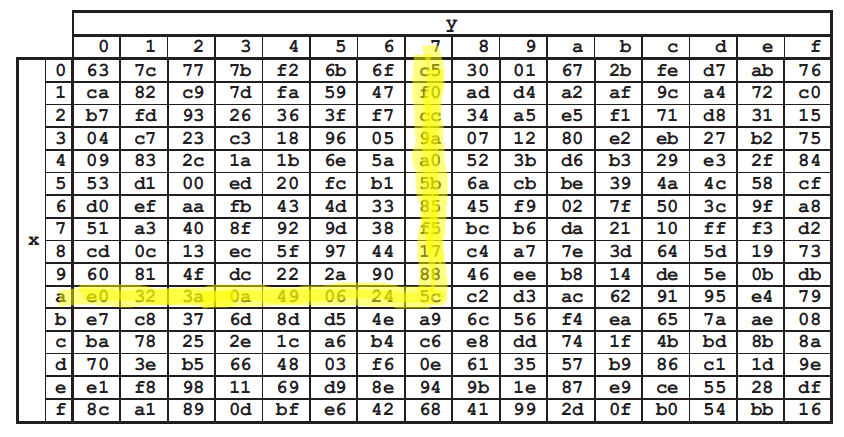
\includegraphics[width=1\textwidth]{Screenshot_6.png}
  \caption{The SubByte S-Box}
  \label{fig:The SubByte S-Box}
\end{figure}

\underline{Result: }S(a7) = (5c)

\newpage
\subsubsection{Compute $S^{-1}$(5c)}

We will try to find on the c = A.b + d formula. In this formula, if a(x) $\neq$ 0 we will compute multiplicative inverse. After, the value found 
will equal to b(x). 
\subsection{Problem 5}

deded








\end{document}










